\documentclass[11pt]{article}
\setlength{\oddsidemargin}{0in}
\setlength{\evensidemargin}{0in}
\setlength{\textwidth}{6.5in}
\setlength{\parindent}{0cm}
\setlength{\parskip}{\baselineskip}


\usepackage{amsmath,amsfonts,amssymb,amsthm,graphicx,tabularx,dblfloatfix}
\usepackage{hyperref}
\usepackage[margin=1.2in]{geometry}

\graphicspath{{./images/} }
\title{\vspace{-7ex}Topological Features of Go Games \vspace{-2ex}}
\author{Edward Kim}
\date{\vspace{-2ex}\today}
\begin{document}
\maketitle

\section{Introduction}
Go, Weiqi, or Baduk is an abstract strategy game where two players compete to enclose and control as much territory as possible on the board. Stones are placed on a board typically consisting of nineteen parallel vertical lines and  nineteen parallel horizontal lines; the stones are placed on the intersections. Players create chains of stones that act as a wall demarcating territory and invade each other's territory both to reduce their opponent's territory and to cement their own. The game's strategic complexity arises from the web of dependencies which appear to be local in scope but global in influence. The centuries of game records and pattern research alone bespeaks of the its hidden labyrinth of complexity.

The difficulty of analyzing the game's strategic dynamics is further evident in the hoary line of trial-and-error pursuits that is Go AI research. As mentioned in the proposal, Go AI have only recently achieved the level of professional play. While Chess AI have performed at professional levels, Go AI have historically only performed at the level of a weak amateaur \cite{bays},\cite{muller}. In addition to the massive search space, many of the moves are deemed illegal. M{\" u}ller  makes the explicit point that only about 1.2\% of all $3^{19 \times 19}$ board configurations are legal configurations \cite{muller}. This puts even more computational strain on an already gargantuan search space. The infeasiblability of creating a half-decent evaluation function to determine the strategic value of any move further compounds the challenge of creating a competent computer player.

However, the seminal victory of the AI player, AlphaGo against 9-dan professional, Lee Sedol became a startling yet monumentous achievement in AI history. Through the techniques of reinforcement learning and Monte-Carlo Tree Search, Google Deepmind was able to create a formidable player which won four out of five matches against Lee Sedol. \cite{alpha} A more recent iteration, AlphaGo Zero, has recently shown even stronger play. The plays from both AI players will be considered in this report.

As mentioned in the proposal, the promise behind using persistent homology on Go games derives from the inherent nature of the patterns arising from the game. Go players frequently create local patterns which are yet part of a set of global patterns on the board \cite{bays}. Tracking these local patterns as the scope becomes broader was one of the major goals pursued by this project. The following revised questions guided the direction of this project:
\begin{itemize}
  \item Can we track the connectivity strength between stone groups changes as the game progresses?
  \item How are games between experienced and inexperienced players different topologically?
  \item Can we determine advantage differentials? As in, can we determine if one player is clearly winning over the other? In particular, do games played by AI exhibit different traits than games played by humans?
\end{itemize}

This report will elaborate on the small successes revealed through TDA techniques and the hurdles which currently preclude deeper analysis of Go games beyond traits seen in the most global scope. All of of the relevant definitions will be explained in the paper as needed.

\section{Basic notions} \label{notions}
As mentioned in the introduction, players place stones of their own color on the intersections of board consisting of nineteen parallel vertical lines and nineteen parallel horizontal lines. Players alternate turns but have the option to forgo their turn. If both players pass, the game ends and the scoring phase commences.

A player's stones are captured if the opponent's stones occupy all adjacent horizontal and vertical intersections. Accordingly, empty adjacent horizontal and vertical intersections are called \textit{liberties}. See Figure \ref{fig:lib1} for an example.

\begin{figure}[ht]
  \centering
  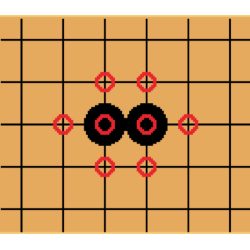
\includegraphics{lib1.png}
  \caption{A simple example of a pair of black stones and its liberties}
  \label{fig:lib1}
\end{figure}

A stones can form extended chains or groups which serve to demarcate territory. A stone group with only one remaining liberty is deemed as \textit{atari} which is considered as imminent for capture. To protect a group from capture, the player must form eyes within a group. Since suicide is illegal, two eyes within a group guarantees life. Referring to Figure \ref{fig:eyes1}, we see that if white were to place any of his or her stones on the red points, it would be considered suicide as black stones completely surround those points. However, if were to imagine only one eye, this black group would immediatly be captured as white would just place a stone on the remaining red point; since the white stones surround the black group, the black group becomes captured.
\begin{figure}[ht]
  \centering
  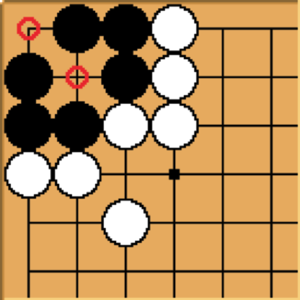
\includegraphics[scale=0.75]{eyes1.png}
  \caption{Two eyes within a group}
  \label{fig:eyes1}
\end{figure}

The \textit{Ko} rule dictates that a board cannot repeat its previous configuration.

\begin{figure}[ht]
  \centering
  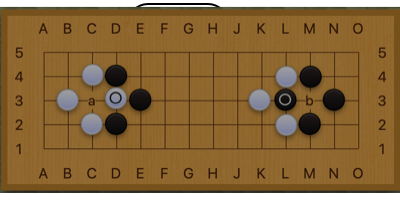
\includegraphics[scale=0.75]{ko1.png}
  \caption{Two eyes within a group}
  \label{fig:ko1}
\end{figure}

There are two types of scoring systems, the \textit{Chinese scoring system} and the \textit{Korean/Japanese scoring system}. In this paper, we will be adopting the Korean/Japanese rules where all of the empty spaces enclosed by one's own stones are counted as well as the number of stones captured. Due to the limitations on scope, this report cannot possibly cover all major Go definitions. The curious reader is referred to \cite{muller} and \cite{terms} for a more complete treatment of the game's rules.

\section{Analysis Engine and Data Sources}

To facilitate proper formulation of ideas for analysis and visualization of persistence diagrams, we developed an extensive analysis engine, TDAGo \cite{tdago}. TDAGo was developed in Python 3 with following libraries:
\begin{itemize}
   \item sgfmill, a SGF game format parsing library
   \item risper and persim, persistent homology libraries
   \item matplotlib, a data plotting library
\end{itemize}

The analysis engine parses the SGF formats and pipes the data into ripser to generate persistence diagrams. It supports a variety of modes including an animation mode for visualizing persistence diagrams for each color as the game progresses. All experiments and persistence diagram plots were created through this engine. The github repository is licensed under the MIT license and is considered open-source. All plots used in this report will be archived in the TDAGo repository.

We use primary use data sources from FoxGoDB \cite{fox} and publicly available AlphaGo archives \cite{alphalib}. All games are transcribed into the universal SGF format for simple retrival.

\section{Basic observations}

We begin with some immediate observations concerning persistence diagrams corresponding to board states. We will reference Figure \ref{fig:lsd1} as needed.
\begin{figure}[ht]
  \centering
  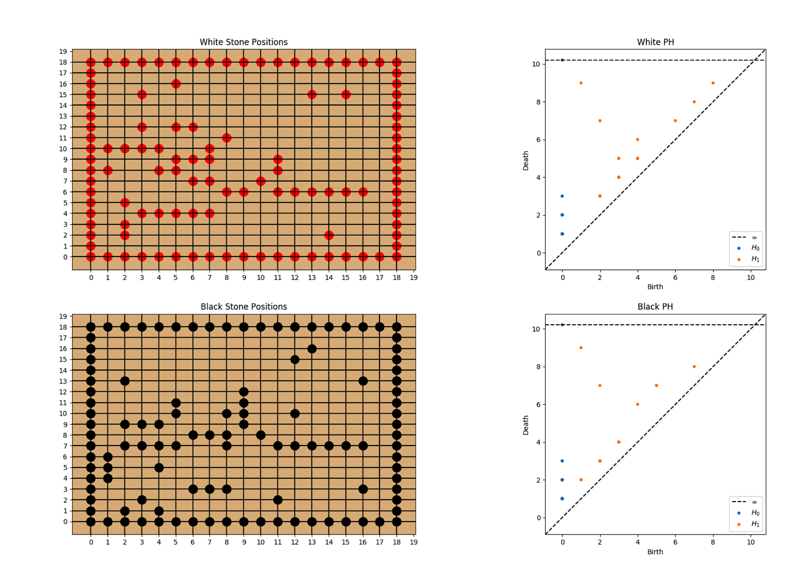
\includegraphics{lsd1.png}
  \caption{The persistence diagrams for the black and white board state for Lee Sedol vs AlphaGo Master: Move 82}
  \label{fig:lsd1}
\end{figure}

Since all adjacent points of intersection on the board are equidistant from one another, every stone's coordinates be a pair of nonnegative integers. Consequently, the birth and death times will both be nonnegative integers as well. We compute our persistence homology cycles by running the library ripser with the Manhatten metric. This metric between two stones has the natural interpretation as the number of subsequent moves a player must make to connect the pair of stones. By observing the behavior of the persistence diagrams as the gane progresses for both players, we come to the following interpretation for the birth and death times:
\begin{itemize}
  \item From the construction of the Vietoris-Rips complex, we can deduce that the birth times will be upper bounds on the number of stones required to connect a pair of consecutive stones along the \textit{boundary}. In other words, to fully enclose the group detected, the player will expect to spend at most $b\cdot n$ consecutive moves where $n$ is the number of stones contained in the detected chain and $b$ is the birth time of the detected chain.
  \item The death times are interpreted as an upper bound on the number of stones required to connect \textit{any} pair of stones in the chain. Once again from the construction of the Vietoris-Rips complex, we can see that any two stones in the chain can be connected by $2d$ stones where $d$ is the death time of the detected chain. Intuitively, we can think of a higher death time as an indication of a larger enclosed area. However, there are some obstacles to this view as we will see later in the report.
\end{itemize}

From these two interpretations, we can start to valuate chains by placing higher value on chains which have lower birth times and higher death times. Lower birth times signify stronger connectivity between the stones in the chain. Stronger connectivity repels any attempt by the opponent to invade and segment the group. Higher death times indicate broadness or a larger span which the chain potentially controls. We proactively used the connectivity data to gauge both human and machine player performance during this project. For many more examples of persistence diagrams of the matches between Lee and AlphaGo Master, we refer the reader to the \href{https://github.com/ekim1919/TDAGo/tree/master/results/LSDAlpha}{Github} repository.

\section{Concerning Connectivity}

As mentioned in the previous section, shorter distances between stones in a chain are desired as such chains are easier to cement into captured territory. For instance, consider the board in Figure \ref{fig:conn1}. Observe the chain of white stones around the center of the board. A cursory glance shows that if the white player desired to complete the chain, he or she will have to spend around three moves to connect one stone of the boundary to the next stone. Compare this to chain of black stones surrounding the aforementioned chain of white stones. Due to the glaring lack of stones at far-left side of the board, the black player must invest more moves to fortify the side. Note that since the white player has higher prospects of completeing his chain, he can use this opportunity to cut the black player's chain in half.

\begin{figure}[ht]
  \centering
  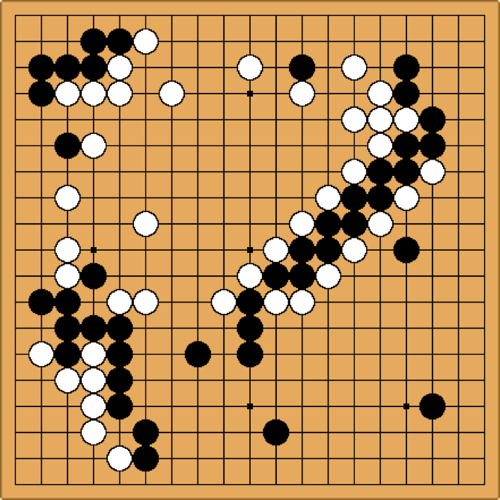
\includegraphics[scale=0.5]{conn1.png}
  \caption{An example board state illustrating connectivity strength between stones}
  \label{fig:conn1}
\end{figure}

These observations inspired us to use connectivity to predict the victor for games played between players of similar rank. The hope was that connectivity would shed a bit of light on the game dynamics seen in novice play in constrast to the presumably more complicated dynamics seen in professional-level play. Through TDAGo, we were able to create a simple connectivity graph by taking the birth times seen for say the black player's board state and simply averaging the birth times of all one-dimensional features detected. Figure \ref{fig:lsdconn1} below illustrates some typical features seen in a connectivity graph. The sharp increase in average distances between stones arises from the nature of Fuseki techniques (opening game techniques). It is a general rule-of-thumb that players should begin to occupy the corners and edges of the board as the boundaries of the board allow for the higher plots of territory for fewer stones. As a result, players' stones tend to be fairly distributed across the board; persistence detects these as weaker features with higher birth times. On the other hand, if we turn our attention to the far end of the graph, we observe that the average distances between the two players begin to converge. The role of the late game properly explains this phenomenon. The late game is understood as a time when all skirmishes have concluded, and all that is left is the task of connecting chains together to formally demarcate territory. Thus, many of the more interesting features detected in a game surface during the middle game where play is mostly dominated by attack and defense tactics rather than territory conquest \cite{terms}. See \cite{terms} for a more comprehensive explanation of the meta-game.

\begin{figure}[ht]
  \centering
  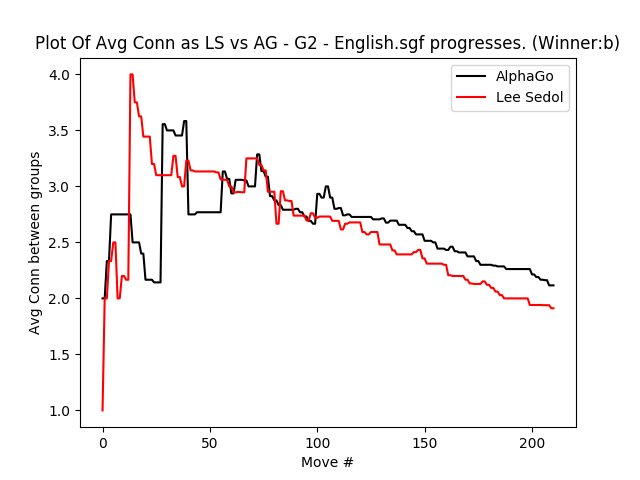
\includegraphics[scale=0.5]{lsdconn1.png}
  \label{fig:lsdconn1}
  \caption{Connectivity graph of the second match between Lee and AlphaGo.}
\end{figure}

To gain a better understanding of the role connectivity plays in games between players of similar rank, we ran the following experiment on 1000 games across a sample of ranks:

\begin{enumerate}
  \item Calculate the average distance between detected chains using TDAGo for each move. We calculate the values separately for each player. That is, the average distance between stones in a black(white) chain will necessarily consist \textit{only} of black(white) stones. Store these results as a time series for each player. Call these time series $B,W$ for the black and white player respectively.
  \item Subtract the two time series $B-W$ in the natural way. Let $S = \int B-W dt$. If $S < 0$, then we predict that black wins. Otherwise, white wins.
\end{enumerate}

This is a rather bare-bones study of determining which player was able to consistently keep his chains tighter than the other during the game. Table \ref{tab:exp} below gives our results. The ranks 20 to 1 kyu refer to increasingly skilled ranks from beginning amateur players to intermediate amateur players. The ranks 1 dan to 9 dan consist of advanced amateur players; above this sysmte is the professional system starting from 1 professional dan to 9 professional dan.

\begin{table}[ht]
    \centering
  \begin{tabular}{|c | c | c|}
      \hline
      Rank & Predictive Accuracy \\
      \hline
      17 Kyu & 58.6\% \\
      \hline
      14 Kyu & 52.6\% \\
            \hline
      7 Kyu &  50.2\% \\
            \hline
      3 Kyu & 52.6\% \\
            \hline
      1 Dan & 46\% \\
            \hline
      Lee vs AlphaGo & 60\% \\
            \hline

      \end{tabular}
      \caption{Results from connectivity prediction experiment for games between human players of fixed rank. Final row includes prediction results for the Lee vs AlphaGo match as well.}
      \label{tab:exp}
\end{table}

The most salient feature to note is the decreasing reliability of connectivity as player skill becomes more sophisticated with the prediction method performing worse than simply flipping a coin on 1 amateur dan games. A possible explanation for this is that inexperienced players cannot defend and attack as well as experienced players as the latter tends have studied the game more deeply. Thus, games between inexperienced players may have more strongly connected chains. Unfortunately, games between players of different rank was more difficult to attain for this project. We hope to extend this experiment to such games to further test the above hypothesis.
\begin{table}[ht]
    \centering
  \begin{tabular}{|c | c | c|}
      \hline
      Game & Predictive Accuracy \\
      \hline
      AlphaGo Master vs. AlphaGo Master & 60\% \\
      \hline
      AlphaGo Zero vs AlphaGo Master & 65\% \\
            \hline
      AlphaGo Zero vs AlphaGo Lee &  90\% \\
            \hline
      AlphaGo Zero vs AlphaGo Zero 20 blocks & 55\% \\
            \hline
      AlphaGo Zero vs AlphaGo Zero 40 blocks & 50\% \\
            \hline
      \end{tabular}
      \caption{Results from connectivity prediction experiment for games between different iterations of Google Deepmind's AlphaGo.}
      \label{tab:mexp}
\end{table}
However, the games played by machines shed further insight on the role of connectivity. We ran the same test on following games between AI players shown in Table \ref{tab:mexp}.

AlphaGo Zero is considered the next iteration of the AlphaGo Master. We note the startling 90\% accuracy for the game of AlphaGo Zero and AlphaGo Lee, the iteration of AlphaGo developed to compete against Lee Sedol in 2016. This game consisted of twenty matches between the two AI; our model was able to predict the victor correctly for eighteen matches. Figure \ref{fig:alphaconn1} shows the glaring disparity between the skill levels of the two computer players. We see that AlphaGo Lee has a strenuous time in the beginning keeping its chains as tightly connected as AlphaGo Zero's chains. The lack of a similar spike in AlphaGo Zero's average distance is worthy of noting. These peculiar behaviors motivate many questions concerning the decision-making procedures made by both computer players as well. A further investigation into AlphaGo Lee's inability to segment AlphaGo Zero's territory effectively is resoundingly warranted but unfortunately outside the scope of this project. Although this experiment is by no means complete or decisive, its results do offer at least intriguing insight into the rising supremacy of AI players over many iterations to come. For the entire archive of connectivity graphs of all matches between AlphaGo Lee and AlphaGo Zero, see the \href{https://github.com/ekim1919/TDAGo/tree/master/results/agzero_vs_aglee}{Github} repository.

\begin{figure}[ht]
  \centering
  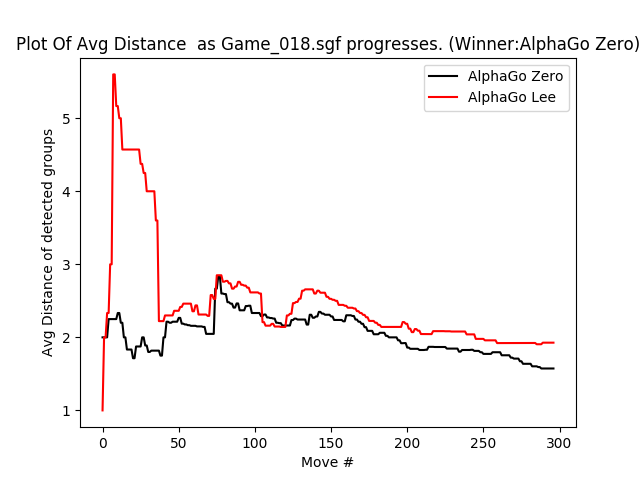
\includegraphics[scale=0.5]{alphaconn1.png}
  \caption{Connectivity graph of the eighteenth match between AlphaGo Master and AlphaGo Lee.}
  \label{fig:alphaconn1}
\end{figure}

\section{Caveats of Territory Estimation}
We have seen in the previous section the natural interpretation of birth times associated to detected features. However, it is not as obvious to interpret the death times. As mentioned in Section \ref{notions}, the death times roughly quantify the ``width" of the enclosed territory. It is tempting to correlate the total area, hence the number of points, with the death times. We will illustate some counterexamples in this section which hinder such a natural definition.

We would like to first remark that it is not difficult to find chains with equal area but are associated to different points on the corresponding persistence diagram. Such a counterexample is portrayed in Figure \ref{fig:counter1}. Although both chains have nine empty interior points, the rectangle above has its point at (1,4) on its corresponding persistence diagram and the thin hexagon below has its point at (2,3). In fact, given a number of desired interior points $17 \geq s \geq 4$, one can extend this example to create a variety of ``skinny and winding" shapes which have area $s$ but different death times. This does not show that all is lost, however. The death times could be useful in finding a \textit{conservative bound} on the area. One possibility is to consider the definition of the Vietoris-Rips filtration and set $(2d)^2$ as the enclosed area where $d$ is the death time. This approximation is conservative at best, and currently it is unclear how to practically utilize the death time to reveal interesting traits about a game.
\begin{figure}[ht]
  \centering
  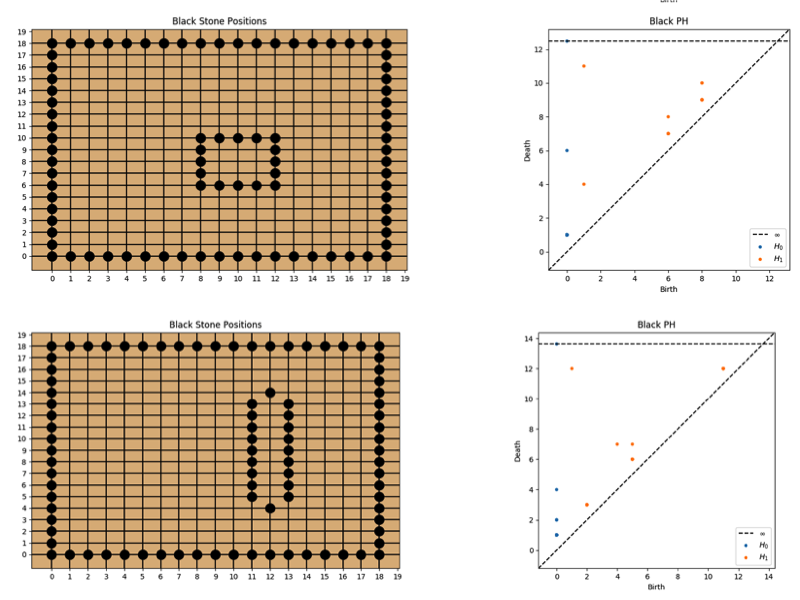
\includegraphics[scale=0.8]{counter1.png}
  \caption{Two chains with equal areas but are associated to different points on corresponding persistence diagrams.}
  \label{fig:counter1}
\end{figure}

A major obstacle to using persistence for territory estimation lies in the set of situations known as \textit{Seki} situations. Seki, or mutual life, refers to a situation where neither stone group can kill the other. These siutations arise as stone groups, especially between opposing players, can share liberties with one other. This is commonly referred to as \textit{mutual liberties}. Consequently, long chains of inter-dependencies can form; some of these dependencies cause a deadlock, hence no player can capture the contested territory. Figure \ref{fig:seki1} illustrates the complexity of some of these Seki situations. The features detected in such a situation would have to be considered moot for persistence to yield a reliable territory estimation method. Currently, this seems highly non-trivial as it unclear that the even simpler task of identifying points on a persistence diagram to its specified feature on the board has an efficient solution.

Seki falls into an even broader category of problems known as \textit{Life-and-Death}. Life-and-Death refers to the status of group as either \textit{alive} or \textit{dead}. Groups that are alive remain on the board indefinitely and groups that are dead become captured by the opponent. These problems form the foundation of a well-rounded Go education and training regime as it challenges players to understand the intricate relationships between stones deeper. The ability to determine the Life-and-Death status of a group allows players to formulate cogent strategies and properly respond to attacks during the middle phase of the game. These fights involve valuating fragile dependencies between large groups of stones; persistence alone is inequipped to handle valuating these dependencies.

\begin{figure}[ht]
  \centering
  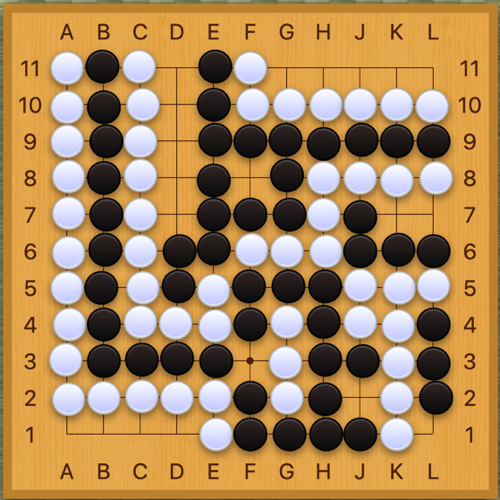
\includegraphics[scale=0.6]{seki1.png}
  \caption{A complicated Seki problem named Hanezeki}
  \label{fig:seki1}
\end{figure}

\section{Further Venues for Development}

Further directions for development fall into two veins. Given more time, we would have liked to pursue further research on the effective use of death times to gauge player performance. This would most likely involve analyzing more shapes to glean more perspective on how the Vietoris-Rips filtration detects topological features. However, we believe that this is the next immediate step for this project. Furthermore, we wish to research implementaions of territory estimation systems which use both persistence and some evaluation function to estimate territory on a local (restricted) section of the board. The hope here is that persistence is simply missing crucial information which can be retrived from some other methodology.

A more involved direction would be to investigate the phenomena exhibited in Figure \ref{fig:alphaconn1}. We would like to first research the reason behind AlphaGo Zero's superiority over AlphaGo Lee in playing ability. These research efforts will aid us in answering the broader question: ``Are most topologically significant features necessarily the most strategically significant features as well?" Answering this question may lead us to immense portions of Go literature and would require a more intimate understanding of the machine-learning techniques involved in training the AlphaGo series. The author does not have much experience with machine-learning whatsoever at this point in time.

Finally, we would like to further develop analysis methods which involve the persistence diagrams of board states involving \textit{both} colors. The analysis used so far only considered board states devoid of the other player's stones. This is an obvious disadvantage that has not been remedied as of yet. However, to properly incorporate the influence from opposing chains, we suspect that persistence diagrams would have to ``cancel'' each other out somehow. In other words, territory claimed by white would have to be penalized based on variables such as proximity from black stones. It is not clear how to achieve this with our current access to software.

\section{Concluding Remarks}
Through our initial efforts, we have seen persistence is fairly effective in determining particular global properties about Go games, namely connectivity. We have shown a small amount of tantalizing evidence that features calculated by current persistence homology libraries can yield perspectives on differences between novice play and professional play. On the other hand, we still run into the issue of undetectable variables influencing the dynamics of global play and vice versa. Even if we know the most prominent topological features on the board, we still must ascertain how these features change as the game progresses. Though we have gained more insight through our efforts, Go still remains extremely difficult to analyze even through a persistence point-of-view.

\bibliography{biblo}
\bibliographystyle{ieeetr}

\end{document}
